\documentclass{article}

\usepackage{color}
\usepackage[margin=1in]{geometry}
\usepackage{graphicx}
\usepackage{hyperref}
\usepackage{listings}

\definecolor{gray}{rgb}{0.5, 0.5, 0.5}
\definecolor{darkgreen}{rgb}{0, 0.6, 0}

\begin{document}
    \raggedright
    Homework 3 \break
    Christopher Seagraves
% % % % % % % % % % % % % % % % % % % % % % % % % % % % % % % % % % % % % % % % 

    \section*{Problem 1}
        \begin{minipage}{\linewidth}
            \raggedright
            I'm sorry, but I protest doing this whole graph. If I deserve partial credit, then so be it, but I'd rather comment my code than manually calculate costs.
            \begin{center}
                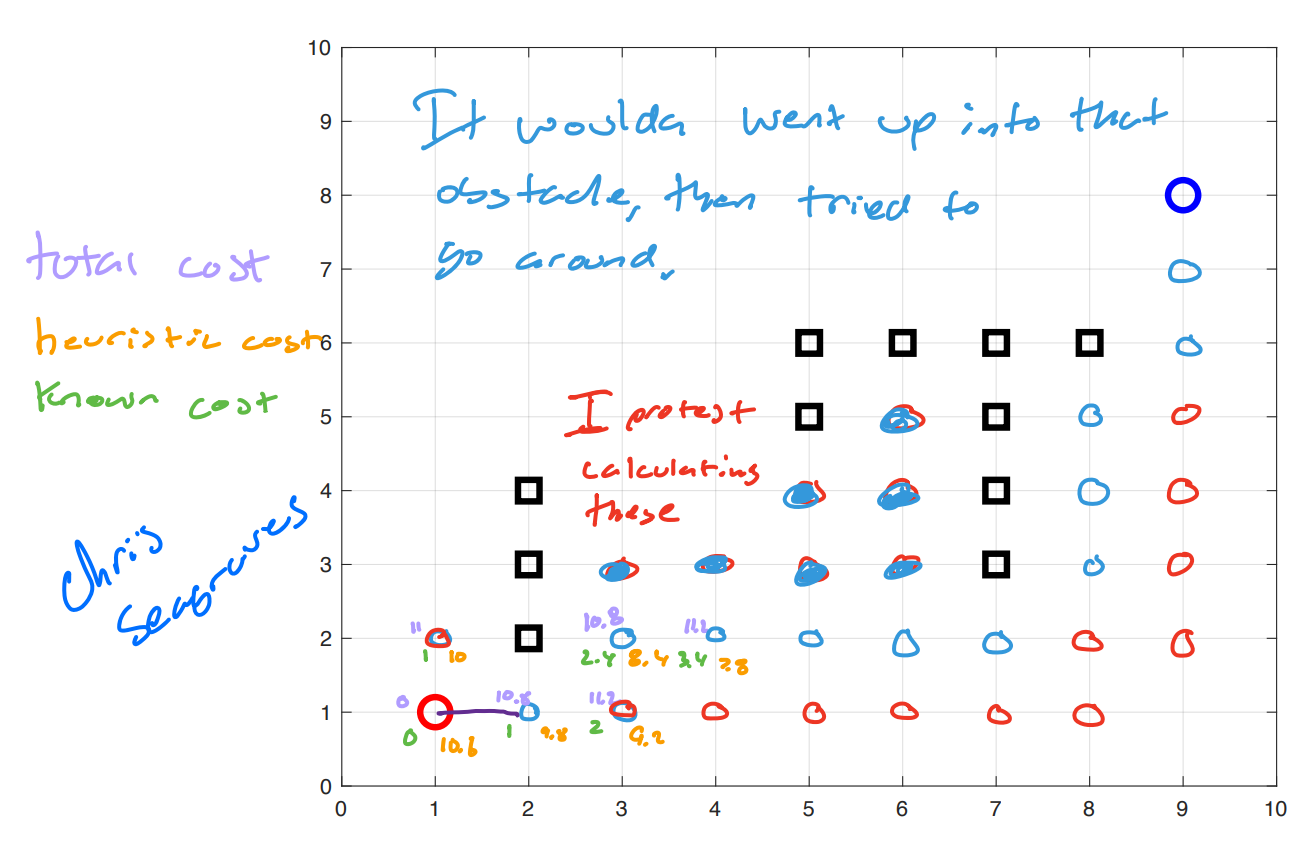
\includegraphics[width=\linewidth]{HW3P1 AStar by hand.png}
            \end{center}
        \end{minipage}
% % % % % % % % % % % % % % % % % % % % % % % % % % % % % % % % % % % % % % % %
    
        \section*{Problem 2}
            \begin{minipage}{\linewidth}
                \raggedright
                It should be noted, if you loop the obstacle list every iteration, this will take a long time - O(nodes-visited * num-obstacles). The solution is to put invalid nodes into a set and check if a given node exists in the set - O(nodes-visited). \break 
                \break
                ./main.py \break
                \url{https://github.com/nosv1/seagraves_unmanned_systems/blob/main/HW3/main.py} \break
                ./AStar.py \break
                \url{https://github.com/nosv1/seagraves_unmanned_systems/blob/main/HW3/AStar.py}
                \begin{center}
                    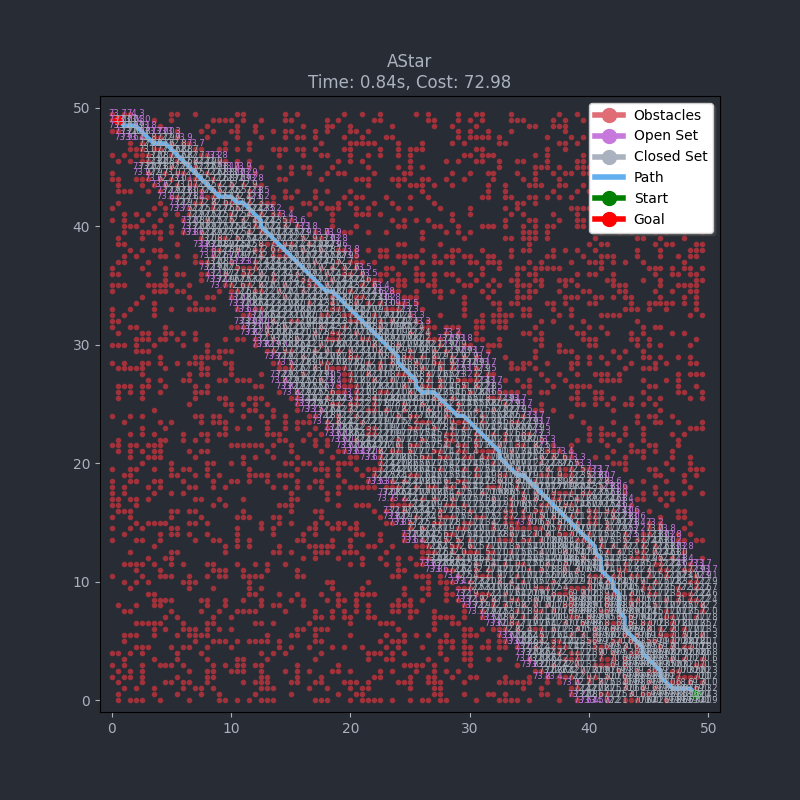
\includegraphics[height=4.5in]{HW3P2 AStar.png}
                \end{center}
            \end{minipage}
% % % % % % % % % % % % % % % % % % % % % % % % % % % % % % % % % % % % % % % % 

        \section*{Problem 3}
            \begin{minipage}{\linewidth}
                \raggedright
                It should be noted, there does not exist a solution if you inflate the obstacles greater than the bot radius. For the plot, I'm plotting the obstacle node at size 0. \break
                \break
                It should also be noted, the algorithim I used for stepping towards a node: \break
                \break
                - generate random node\break
                - step towards node from closest node \break
                - check if snapped-to-grid sub-steps along step are valid \break
                - saving node if step is valid \break
                \break
                This lets me use steps that aren't in the grid but check if nodes are valid quickly. Like, for a more relaxed map - with more space between obstacles - I can inflate an obstacle, define the nodes in the obstacle as invalid, snap to a close node, check if it's invalid, and assume my 'non-snapped' node is valid or invalid.\break
                \break
                Something else to consider about taking steps towards nodes and using 'non-snapped' nodes is - assuming your obstacle is equa-distant to its center - take sub-steps along your step to see if any of them are invalid; this helps to avoid stepping over part of an obstacle - even if your close node and new node are both valid. However, checking sub-steps bumps the time from O(nodes-visited) to O(nodes-visited * sub-step-ratio). \break

                RRT is terrible for goals close to the edge... It's just luck if the randomizer generated points beyond the edge to step towards the goal... I wound up expanding my randomizer range to 1.5x the map size to help it.
                \break
                ./main.py \break
                \url{https://github.com/nosv1/seagraves_unmanned_systems/blob/main/HW3/main.py} \break
                ./RRT.py \break
                \url{https://github.com/nosv1/seagraves_unmanned_systems/blob/main/HW3/RRT.py}
                \begin{center}
                    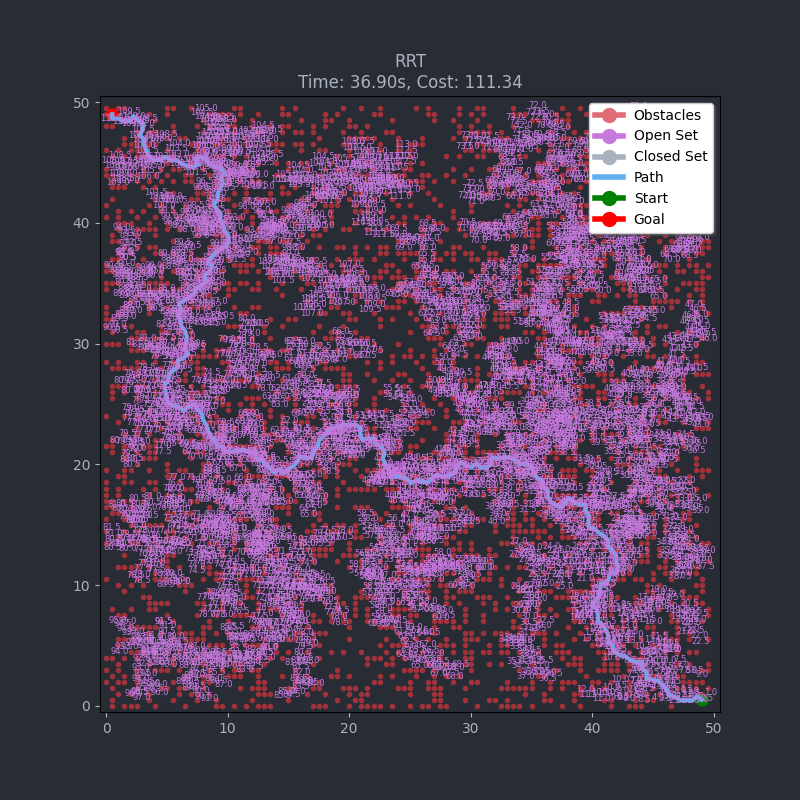
\includegraphics[height=4.5in]{HW3P3 RRT.png}
                \end{center}
            \end{minipage}
% % % % % % % % % % % % % % % % % % % % % % % % % % % % % % % % % % % % % % % % 

\end{document}